% ====================
\chapter{Method (My Idea)}
% ====================

% • In a paper you MUST provide the details, but FIRST convey the idea
% • Introduce the problem, and your idea, using EXAMPLES and only then
% present the general case
% • Explain it as if you were speaking to someone using a whiteboard
% • Conveying the intuition is primary, not secondary
% • Once your reader has the intuition, she can follow the details (but not vice
% versa)
% Even if she skips the details, she still takes away something valuable
% Evidence
% • Your introduction makes claims; The body of the paper provides evidence to
% support each claim
% • Check each claim in the introduction, identify the evidence, and forward-
% reference it from the claim
% • Evidence can be: analysis and comparison, theorems, measurements, case
% studies

% ====================
\section{My Idea (2 pages)}
% ====================

% ====================
\section{The details (5 pages)}
% ====================

% ====================
\chapter{Motion Planning}
% ====================
% --------------------
\section{Basic Ingredients}
% --------------------
\begin{itemize}
\item State
\item Time
\item Actions
\item Initial and Goal States
\item Feasibility and Optimality Criterion
\item A Plan
\end{itemize}

For a full description, see Chapter 1.3 of Lavalle \cite{lavalle2006planning}.
% --------------------
\section{Introduction to Motion Planning}
% --------------------
% --------------------
\subsection{Simple Motion Planning}
% --------------------
The simplest motion planning problems assume knowledge of a global map, a fixed
known goal state and a fixed known initial state. The problem is to determine a
feasible path from the initial state to the goal state. An optimality criterion
may also be applied to choose the best path if multiple feasible ones are found.

Notably, two important concepts have often been ignored in determining the path:
the dynamics of the system and the use of feedback. Dynamics refers to how
states transition to other states, and is inherent in real-world systems. For
example, a car can easily move fowards and backwards, but cannot immediately
move side to side. Feedback refers to the technique of refining further actions
based on newly sensed data. In simulations, feedback may not be necessary, but
in real-world systems, errors in sensing and modeling build up over time without
it.

In this simple case, the generated path is followed in an open-loop manner, or
if subject to real-world constraints (see \autoref{fig:lavalle2006planning119}),
the generated path is smoothed to obey the system's dynamics and feedback is
used to closely follow the path. "Notably this approach is highly decoupled as
feedback and dynamics are neglected in constructing the original path"
\cite{lavalle2006planning}. The smooth path may now obey the robot's dynamics,
but may no longer be feasible.  Feedback is used merely as an inefficient
afterthought.

\begin{figure}
\centering
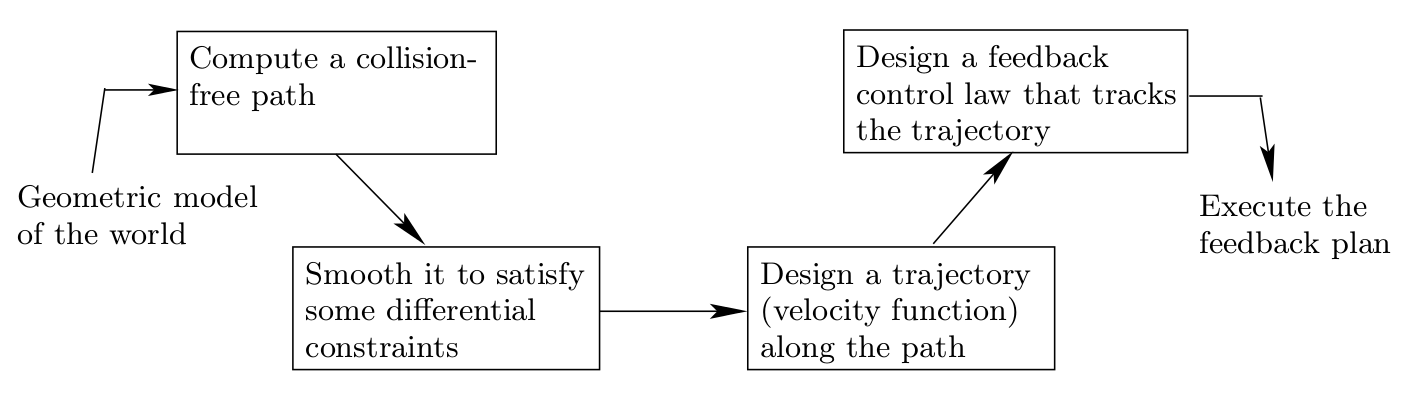
\includegraphics[width=3in]{figures/lavalle2006planning119.png}
\caption{From \cite{lavalle2006planning}. A refinement approach that has been used for decades in robotics.}
\label{fig:lavalle2006planning119}
\end{figure}

Even in this simple case, obtaining an optimal or even feasible path is not
straightforward if the state space is large. A* search for trivially sized state
spaces and sampling-based techniques such as RRTs (RRT* for optimality) and PRMs
have proven to be the methods of choice (citation?), though it is still an
ongoing field of interest (cite 2015 RRT/PRM papers).

% --------------------
\subsection{Feedback Motion Planning}
% --------------------
Dynamics refers, generally, to how a state transitions to another state.

Feedback (or reactive plans) refers to something else.

Tiers of motion planning problems
\begin{itemize}
\item Fixed Initial and Goal States, no dynamics, no feedback, some optimality
criterion: RRT*, PRM*
\item Fixed Initial and Goal States, dynamics, no feedback: RRT*, A*
\item Fixed Initial and Goal States, no dynamics, feedback
\end{itemize}

see \autoref{fig:determinedrive2}.
\begin{figure}
\centering
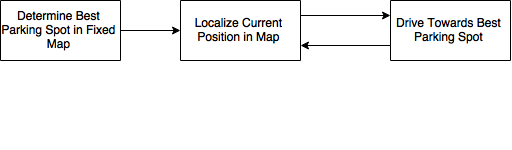
\includegraphics[width=3in]{figures/determinedrive2.png}
\caption{Feedback loop}
\label{fig:determinedrive2}
\end{figure}


% --------------------
\subsection{Feedback Motion Planning with Updating Goal State}
% --------------------
see \autoref{fig:determinedrive1}.
For a full description, see Chapter 8 of Lavalle \cite{lavalle2006planning}.

\begin{figure}
\centering
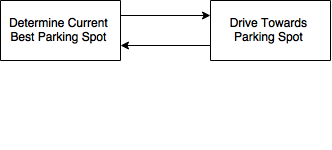
\includegraphics[width=3in]{figures/determinedrive1.png}
\caption{Feedback loop}
\label{fig:determinedrive1}
\end{figure}

